\usetikzlibrary{patterns}



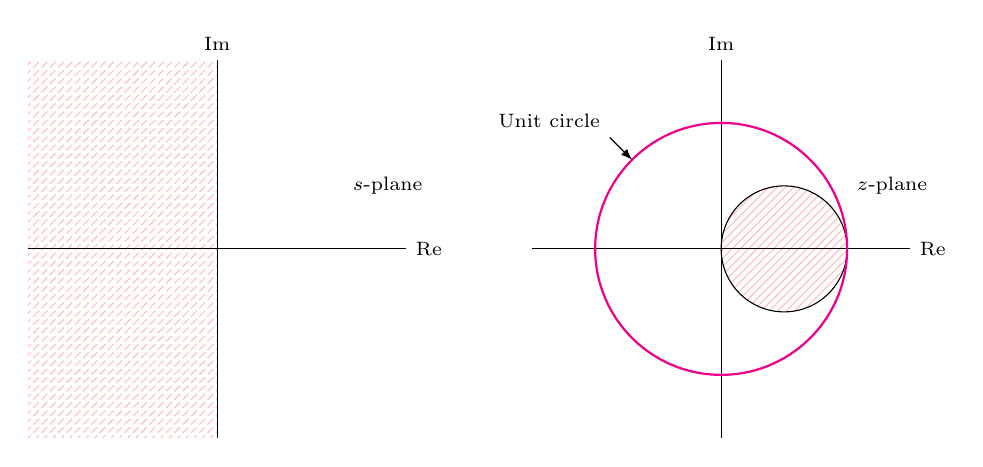
\begin{tikzpicture}[scale=0.8]



    	\begin{scope}
     		\path [dashed, pattern color=pink, pattern=north east lines] (-11, -3)  rectangle ++(3, 6);
	\end{scope}
    \draw (-11, 0) -- (-5,0) node[anchor=west] {\scriptsize $\mathrm{Re}$};
    \draw (-8, -3) -- (-8,3) node[anchor=south] {\scriptsize $\mathrm{Im}$};
    \node at (-6, 1) [anchor=west] {\scriptsize $s$-plane};    

    \def\pole{++(135:0.1) -- ++(-45:0.2) ++(135:0.1) -- ++(45:0.1) -- ++(-135:0.2) +(45:0.1)}
    \def\zero{circle (0.1)}
    	\begin{scope}
     		\path [draw=black, pattern color=pink, pattern=north east lines] (1, 0)  circle (1);
	\end{scope}

    \draw (-3, 0) -- (3,0) node[anchor=west] {\scriptsize $\mathrm{Re}$};
    \draw (0, -3) -- (0,3) node[anchor=south] {\scriptsize $\mathrm{Im}$};
    %\pause
    \draw[thick, magenta] (0,0) circle (2);
    \draw [latex-] (0,0) ++(135:2) -- ++(135:.5) node [anchor=south east] {\scriptsize Unit circle};

    \node at (2, 1) [anchor=west] {\scriptsize $z$-plane};
    %\draw (2, 0) node[anchor=north west] {$1$} \pole;
    %\draw (1/3, 0) node[anchor=north ] {$\frac{1}{3}$} \pole;
	%\draw    (0,0) \zero;
\end{tikzpicture} 